\newcommand{\st}{ \ | \ }

\section{Requirements for New Graph Syntax}
  \label{s:requirements}
  The ultimate goal of the new graph--based syntax presented here is to be able to 
  fully describe the general structure of an MDAO problem independently of any solution information, 
  while still being able to accomodate the more specific case when a solution 
  strategy is applied. In order to achieve that goal 
  the graph needs to accomodate a number of constructs of MDAO problems: 
  \begin{itemize}
    \item Analysis tools and connections between them
    \item Design variables, objectives, and constraints
    \item Local and global properties
    \item Coupling between analyses
    \item Multi-fidelity analyses
  \end{itemize}

  Beyond those basic constructs, there are also three phases of a design process that 
  all need to be representable with the new syntax. Firstly there is the initial problem definition
  phase where the specific analysis tools and design goals are identified. At the end of this phase, 
  a single formal problem formulation is selected specifying design variables, constraints, objectives, 
  analysis tools, etc. Lastly some specific procedure for solving the problem is selected, for example 
  picking an MDAO optimization architecture. Using the proposed graph syntax, each of these phases 
  can be represented with the following three graphs:
  \begin{itemize}
    \item Maximal Connectivity Graph (MCG)
    \item Fundamental Problem Graph (FPG)
    \item Problem Solution Graph (SPG)
  \end{itemize}

  The \emph{maximal connectivity graph} represents the first phase with all 
  analysis codes being considered and all possible connections between them also present. The second graph 
  is the \emph{fundamental problem graph}, which is the smallest possible graph 
  that still fully defines a given problem formulation. Finally, a \emph{specific problem formulation} 
  may be represented by including additional edges and nodes to represent the 
  solution strategy being employed to solve the problem. 

  The relationship between these three graphs is depicted in Figs.~\ref{f:tree} and \ref{f:hourglass}. 
  The tree diagram demonstrates the fact that it is generally possible to obtain 
  multiple FPGs from a single maximal connectivity graph. This  may correspond to 
  different down--selections of analysis codes, different connections between them, 
  or both. Each down--selection shrinks the number of possible FPGs that could be reached 
  until only one is remaining. Then, from a single FPG, different PSGs may be obtained by implementing 
  different solution strategies. If you consider the size of a graph to be the sum of all of its
  edges and nodes then the hourglass shape in Fig. \ref{f:hourglass} illustrates how
  the MCG gets reduced to a single FPG, then multiple possible PSGs exist to solve the problem.
  In other words the FPG is obtained from the MCG by removing nodes and edges, 
  and the PSG is obtained from the FPG by adding nodes and edges.

  \begin{figure}[htb!]
    \centering
    \subfigure[number of possible graphs]{
    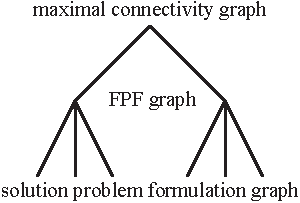
\includegraphics[width=2.0in]{images/tree}
    \label{f:tree}
    }
    \subfigure[graph size]{
    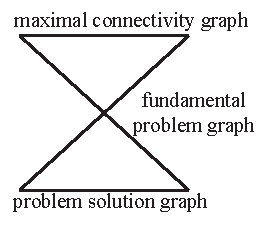
\includegraphics[width=2.0in]{images/hourglass}
    \label{f:hourglass}
    }
  \caption{The relationship between the MCG, FPG, and PSG.}
  \end{figure}

\section{Syntax Definition}
  \label{s:syntax definition}
  In this section we present the necessary graph theory fundamentals to 
  construct the graphs discussed above. 
  The notation used in this work is adapted from Diestel \cite{Diestel2010}. 
  A \emph{graph} is a pair $G = (V,E)$ of sets such that $E \subseteq V \times V$, 
  which means that the elements of $E$ are 2--element subsets of $V$. The set $V$ 
  contains the \emph{vertices} or \emph{nodes} and the set $E$ contains the \emph{edges}.
  For a \emph{directed graph*} (or \emph{digraph}) we construct $E$ as a set of ordered pairs instead 
  of a set of sets. Each ordered pair represents an edge starting at the node 
  indicated by the first entry and directed to the node indicated by the second 
  entry. Edge $e$ = $(x,y)$ may be referred to simply as $xy$. For node $v \in V$ 
  the edges directed out are given by $E(v)$ and the edges directed into $v$ are given 
  by $E^{-1}(v)$; $E(E(v))$ is denoted as $E^2(v)$, and likewise for additional levels. 
  If $E$ is not a one--to--one mapping, $E(v)$ may be the empty set, a single node, or a set of nodes.
  \begin{figure}[htb!]
    \begin{center}
    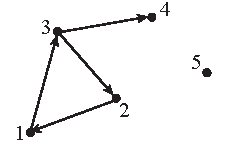
\includegraphics[width=1.5in]{images/example_directed_graph}
    \end{center}
    \vspace{-20pt}
  \caption{Example directed graph.}
  \label{f:example directed graph}
  \end{figure}
  As an example, for the directed graph shown in Fig.~\ref{f:example directed graph} we have
  \begin{IEEEeqnarray*}{rCl}
  V & = & \{1,2,3,4,5\}, \\
  E & = & \big\{(1,2),(3,2),(1,3),(3,4)\big\}.
  \end{IEEEeqnarray*}

  A \emph{path} $P=(V,E)$ from $x_0$ to $x_k$ in graph $G$ is a subgraph of $G$ with $V = \{x_0,x_1,\ldots,x_k\}$ and $E = \{(x_0,x_1),(x_1,x_2),\ldots,(x_{k-1},x_k)\}$.
  A \emph{reverse path} $P_R$ in graph $G$ is a path on $R$, where $R$ is the reverse graph of $G$ obtained by switching the orientation of every edge.


  %does this belong in the analysis block section???? 
  Let $I$ be a nonempty set of counting numbers such that for each $i \in I$ there is a corresponding set $A_i$. 
  The set of sets $\mathcal A = \{A_i \st i \in I\}$ is called an indexed family of sets with index $i$ and 
  indexing set $I$\cite{smith2006}. 
  The union over this family of sets can be described in a few different ways:
  \begin{equation}
  \bigcup_{i \in I} A_i = \bigcup_{A \in \mathcal A} A = \{x \st x \in A \txt{ for some } A \in \mathcal A\}.
  \end{equation}

  Lastly, the cardinality of a set $B$ is the number of elements in $B$ and is denoted as $|B|$.

\subsection{Node and Edge Types}
  \label{ss:types}
  We now define different types of nodes and edges with specific properties to compose graphs used to represent an MDAO problem. 
  There are three node types:  
  \begin{description}
  \item[variable: ] represents scalar or array data
  \item[model:] responsible for mapping inputs to outputs
  \item[driver:] control logic capable of managing iteration
  \end{description}

  In addition to the three node types, there are two edge types: 

  \begin{description}
  \item[connection edge:] Exchange of information between two nodes. These edges 
  can either be fixed (can not be removed from graph) or free (can be removed). ((this needs to be modified, as analysis blocks cannot be altered but they can be removed as a group))
  \item [implicit edge:] Implicit passing of information from a driver node to a 
    variable node. A single variable node can have many incomming implicit edges. These edges are 
    free and can be added or removed from the graph. 
  \end{description}

  [[Insert legend for node and edge types]]

  In Alexandrov and Lewis's REMS syntax only two node types were present, variable 
  and function, and only one edge type\cite{alexandrov2004}. We've chosen to rename the ``function'' node 
  type to ``model'' to be more consistent with modern MDAO frameworks. The present work 
  adds two more node types and one more edge type to the syntax to allow descriptive
  graphs for all three phases of the design process. 

\subsection{Rules for Nodes and Edges}
  \label{ss:rules}
  There are specific rules for the usage of these nodes and edges.
  The driver node and the implicit edge are only allowed to be present in PSGs. All 
  other node and edge types can be present in any of the three graphs, subject to these restrictions: 
  \begin{enumerate}
  \item A model node can only have one edge directed to or from another model node.
  \item A model node can only have fixed connection edges directed in or out.
  \item A model node must have at least one edge directed in and at least one edge 
    directed out.
  \item If a variable node has an outgoing edge to a model node then it may not have 
    any other outgoing edges.
  \end{enumerate}

\subsection{indegree and outdegree}
  \label{s:indegree-outdegree}
  The \emph{indegree} of a node is the number of connection edges directed in and 
  is denoted as $\txt{deg}^-(v)$, and the \emph{outdegree} 
  is the number of connection edges directed out and it is denoted as $\txt{deg}^+(v)$.
  The degree of a given node is only a function of the connection edges 
  attached to it. The number of implicit edges is not relevant since any number 
  of drivers could be involved, at different parts of an solution process. For 
  example in a sequential optimization where a global optimizer is first applied
  and a gradient based one is applied second, design variables would have incomming 
  implicit edges from both optimizers but this would not affect the indegree of those
  variable nodes. 
  ((DP:I started to remove any reference to the edge type in these definitions but then saw that you needed it. The reason I did that was because indegree and outdegree are basic graph theory terms. What if the reference to implicit edges is handled with the upper indegree limit, i.e. after the FPG is obtained the upper indegree limit for the design variable nodes is relaxed (increased) so that it isn't a problem what is or isn't counted?))

  We also define the \emph{upper indegree limit} 

  \begin{equation}
  \txt{deg}_u^-(v):V \to \mathbb{N}
  \end{equation} 
  and the \emph{lower indegree limit} as
  \begin{equation}
  \txt{deg}_l^-(v):V \to \mathbb{N}.
  \end{equation}
  These user-specified limits govern the number of connection edges that may 
  be directed into a variable node for a valid graph. Consider a variable 
  node $v$ with $\txt{deg}_u^-(v) = \txt{deg}_l^-(v) = 1$. In this case, $v$ 
  must have exactly one incomming explicit edge or the graph is invalid. 
  Two possiblities exist for voilating these limit conditions: 

  \begin{description}
    \item[hole: ] The number of incomming edges is less than the lower indegree limit:
      \begin{equation} \txt{deg}^-(v) < \txt{deg}_l^-(v) \label{e:hole} \end{equation}
      This represents a lack of information being supplied to the node.
    \item[collision: ] The number of incomming edges is greater than $ \txt{deg}_u^-(v)$. 
      \begin{equation} \txt{deg}^-(v) > \txt{deg}_u^-(v) \label{e:collision}\end{equation}
  \end{description} 

  An algorithm for detecting and managing these violations if proposed in Sec.~\ref{s:building graphs}.\ref{ss:obtaining FPG}.

\section{Graph Representation of MDAO Constructs}
\label{s:graph representation}
In this section we will make use of the Sellar problem, described in 
Eqn. \ref{eqn:simple_fpf}. The graph representation of the Sellar problem, 
using the new stynax, is presented in Fig. \ref{f:sellar_graph_full}. Throughout
the rest of this section, different sub-graphs or slight modifications of 
the full graph will be used to demonstrate the important MDAO constructs within
this graph syntax.

\begin{figure}[htb!]
    \begin{center}
    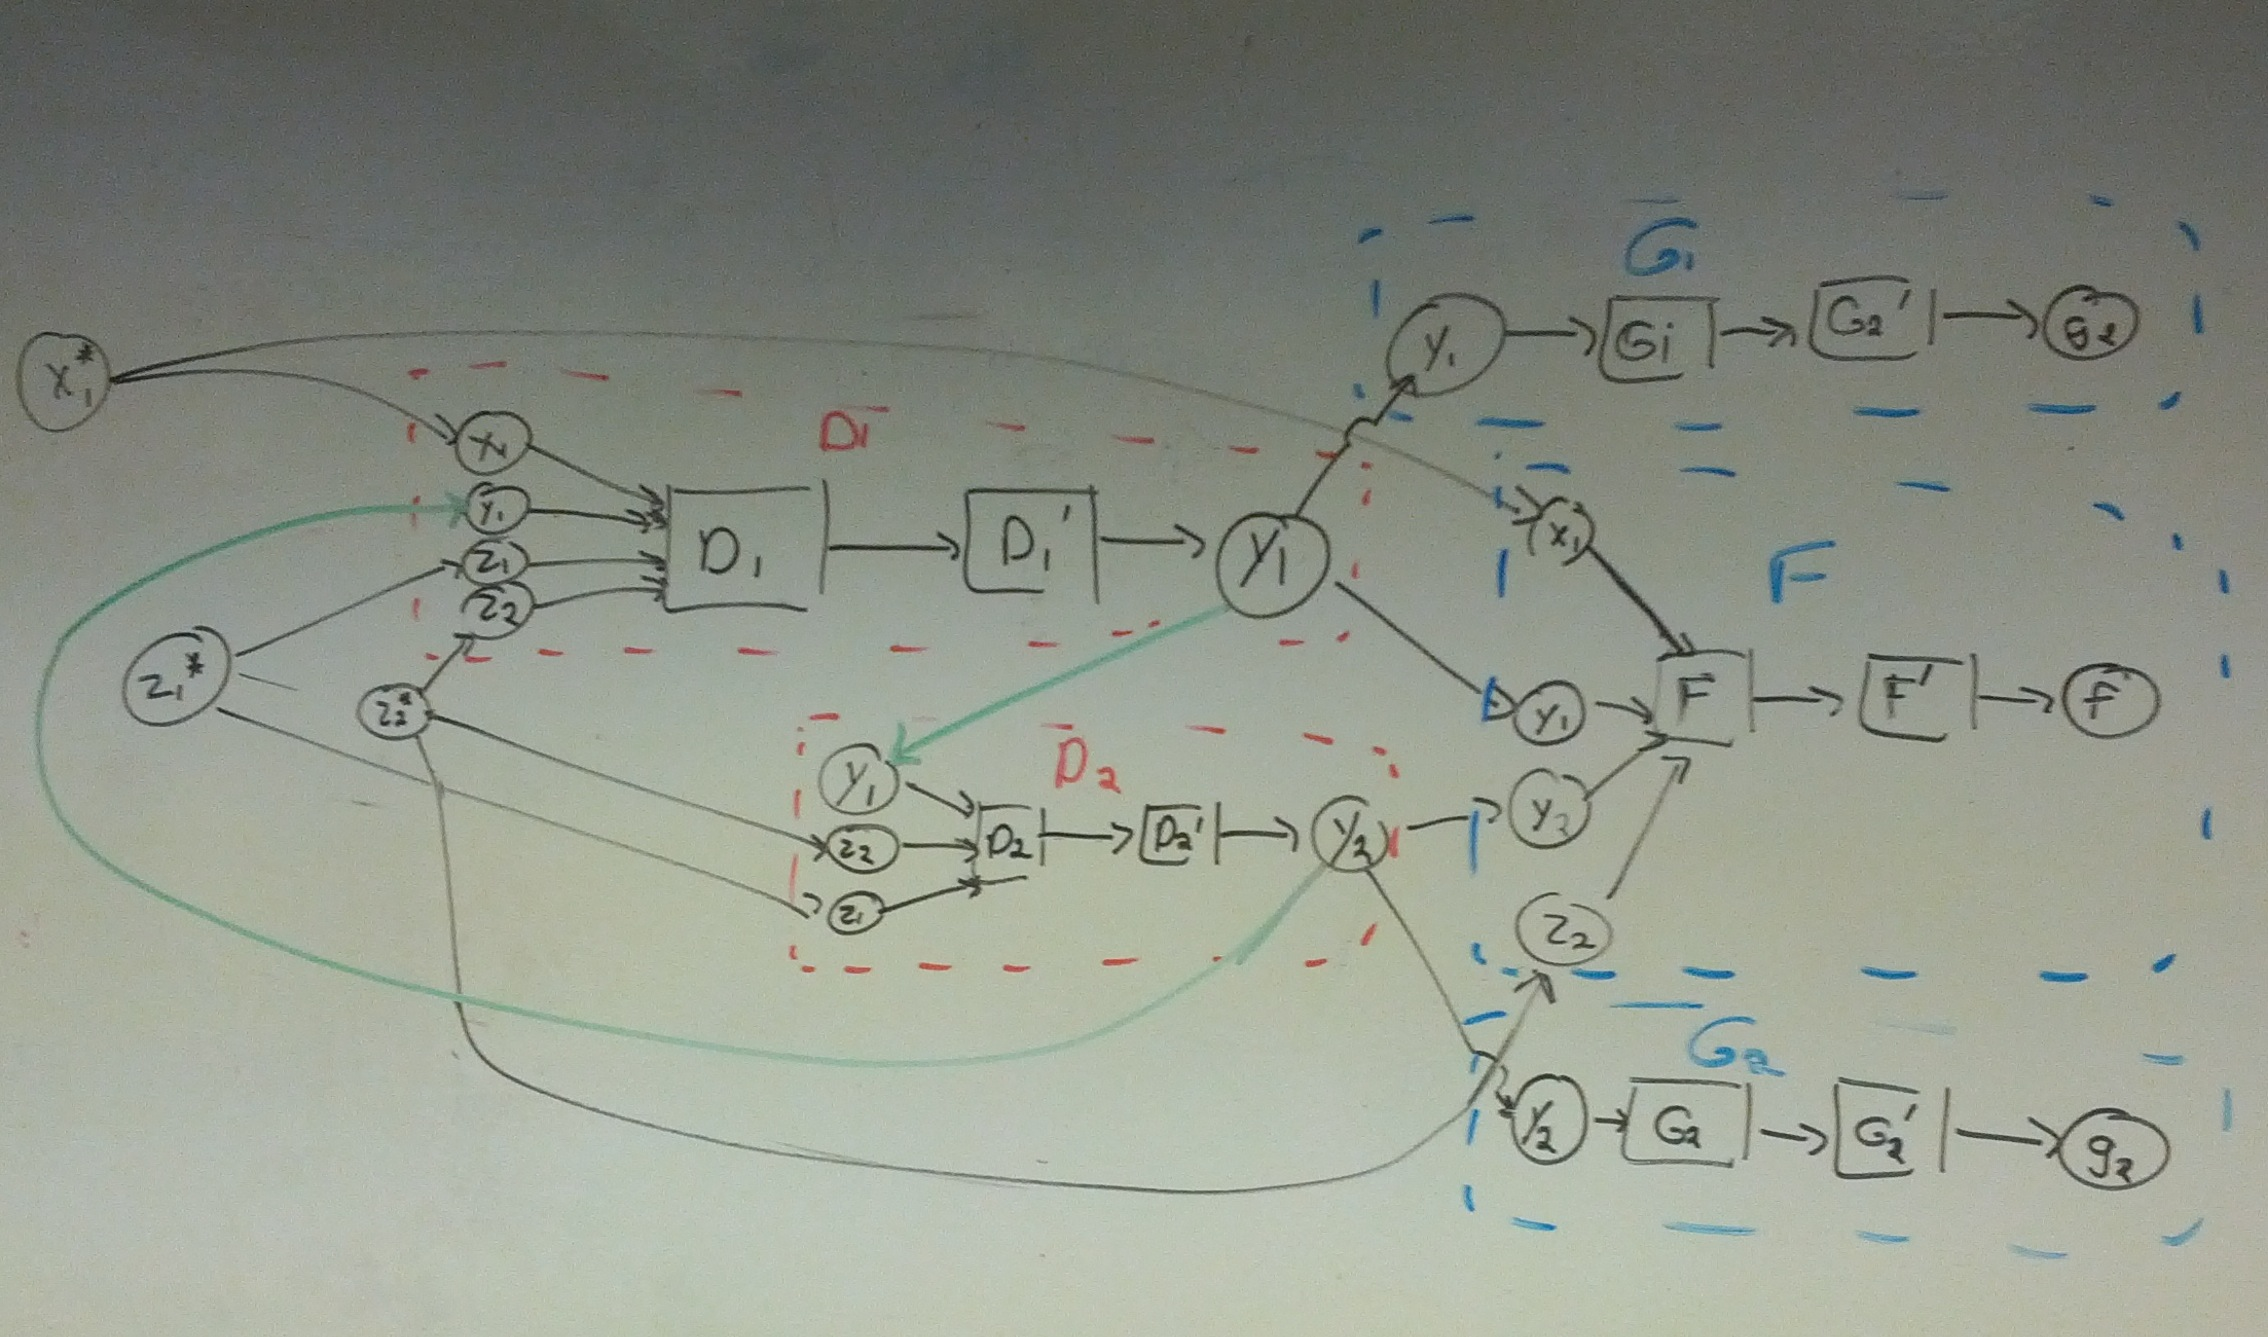
\includegraphics[width=4in]{images/sellar_graph_full}
    \end{center}
    \vspace{-10pt}
\caption{Graph of the Sellar problem formulation}
\label{f:sellar_graph_full}
\end{figure}

\subsection{Analysis Blocks and Connections}
\label{ss:analysis blocks and connections}
Analysis tools take in a number input variables and then perform some work to calculate 
the values for their respective outputs. In an MDAO graph, this process is 
represented by a group of nodes and edges called an \emph{analysis block}, 
shown in Fig. \ref{f:analysis block}. Within an analysis block each variable 
node represents a single input or output and is connected 
to a single model node via a fixed edge. Note that in Fig.~\ref{f:analysis block}, 
the analysis block contains two model nodes, with a single edge connecting them. 
This edge represents the necessary calculations to map given inputs 
to proper output values. If constructing a weighted graph, the weight calculation edge 
provides the opportunity to computational cost. However, it is also allowed to 
skip this edge and have both incomming and outgoing edges to variables through a 
single model node for a given analysis block. Although analysis blocks are 
comprised of multiple nodes and edges, since all the edges within them are 
fixed, they become fixed sub-graphs within a graph. In this way, they cannot be 
altered but they can be removed as a group.

\begin{figure}[htb!]
    \begin{center}
    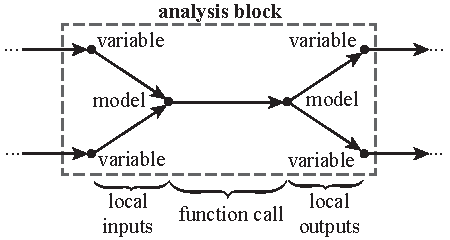
\includegraphics[width=4in]{images/analysis_block}
    \end{center}
    \vspace{-10pt}
\caption{Example analysis block. The each node type and edge type is labeled in italics and annotated parenthetically.}
\label{f:analysis block}
\end{figure}

Variable nodes in an analysis block can be distinguished as either an input or 
an output by the manner in which they are connected. As shown in Fig.~\ref{f:analysis block}, 
inputs are any variable nodes that have an outgoing edge into a model 
node. Conversely, outputs are any variable nodes that have an incoming edge from a model node. 

MDAO problems require that information be passed between sets of analyses. When 
information from the output of one analysis block is passed, or connected, to the 
input of another analysis block, a new connection edge is added connecting the two 
variable nodes involved in the exchange. These connection edges are free, unlike the edges 
within an analysis block, can be added or removed depending on the needs
of a given design problem. In other words, free connection edges are created by 
engineers linking the output of one tool to the input of another one. Note that 
it is allowed for a single output to have outgoing connection edges to multiple 
downstream inputs. 

\subsection{Design Variables}
((DP:I'm thinking we might also need the upper indegree limit to be zero as well, because setting only the lower indegree limit makes the node a design variable if it didn't have any incoming edges. It's seems possible that in the MCG a node has incoming edges but the user wants it to be a design variable. I can make the change if you agree.))
For the Sellar problem, there are three design variables, $x_1^*$, $z_1^*$, and $z_2^*$. In Fig. 
\ref{f:sellar_graph_full}, these are the only three holes (nodes without out 
incomming edges) in the graph. 

\begin{figure}[htb!]
  \begin{center}
  [NOTE: Re-work this one to match $D_2$ from Sellar]
    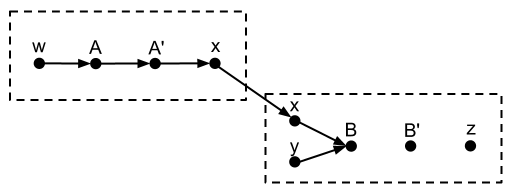
\includegraphics[width=.6\textwidth]{images/design_vars_graph}
  \end{center}
  \caption{Notional graph with two potential design variables \label{f:designvars}}
\end{figure}

More formally stated, given a MCG with the $\txt{deg}_l^-(v)=1$ for all nodes, 
there will likely be a set of holes preventing a valid FPG from being obtained. 
Each hole represents a node that could potentially become a design variable. 
It is up to the designer to examine each and decide if it is appropriate to 
consider it a design variable, in which case the designer shall set the lower 
indegree limit to be zero. However, some variable holes may not actually be 
suitable as a design variable. For instance, if an aircraft mission analysis 
code requires a drag input which ends up being a hole then it's likely best to 
leave$\txt{deg}_l^-(v)=1$ and find a new analysis code to fill the hole in graph. 

So a design variable is defined as any variable node with $\txt{deg}_l^-(v)=0$. 
This, by definition, means that design variables are not holes in the graph, since 
they have not violated their lower indegree limit. Regardless, 
when working with a MCG or FPG, only connection edges are allowed, so a design 
variable in either graph will be a variable with no incomming edges edges. For a valid PSG 
any design variable node would have at least one, but possibly multiple, incomming 
implicit edges from one or more driver nodes. 

\subsection{Objectives, and Constraints}
\label{ss:objectives and constraints}
Like design variables, objectives and constraints are also constructs that need 
to be identified when setting up a given design problem. In the case of 
objective functions single output values could be selected, but commonly multiple 
values are assembeled together via simple algebraic expressions to form a composite 
objective function. (e.g. The objective function from Eqn. \ref{eqn:simple_fpf} is
$x_1^2+z_2+y_1+e^{-y_2}$). Constraints are always given in the 
form of either an inequality or an equality. (e.g. a constraint from Eqn. 
\ref{eqn:simple_fpf} is $\frac{y_1}{3.16}-1\geq0$.) By convention, 
constraints are usually given such that some expression will be less than or equal 
to zero, so any positive value would violate the constraint. For both objective 
and constraints, these simple expressions take some inputs and map them to an
output value of significance to the overall design problem. 

These operations, though very simple, are effectively the same kind of task 
performed by an analysis block. A constraint or objective function can therfore 
be represented as another analysis block on the graph, with it's own input and 
output variable nodes. Although fundamentally no different than an analysis block, 
for clarity and convience it is useful to distinguish between regular analysis 
blocks and those that arise from the addition of objectives or constraints to 
the graph. Therefore, we define an \emph{expression block}, as the collection of variable and model 
nodes related to a given objective or constraint function. Fig. \ref{f:obj-cons}
highlights the objective and constraint blocks from the Sellar problem. 



\begin{figure}[htb!]
  \begin{center}
    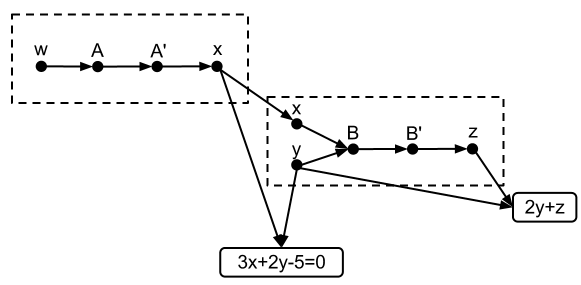
\includegraphics[width=.6\textwidth]{images/obj_const_graph}
  \end{center}
  \caption{Notional graph with and objective and constraint nodes \label{f:obj-cons}}
\end{figure}


\subsection{Local vs Global Nodes}

  A simple definition of a global node is any node that involves information 
  from more than one analysis block. Likewise, a local node is any node 
  that involves information from only a single analysis block. As stated before, variable 
  nodes with fixed edges directed to model nodes (as part of an analysis block) are inherently local 
  and similarly model nodes are also local. Global variables are a part of many 
  MDAO problems and must be representable in the graph. Follwoing our simple definition
  any variable node that had multiple incomming or outgoing edges, would be global. 
  In Fig. \ref{f:sellar_graph_full} the variable nodes for $x_1^*$, $z_1^*$, and $z_2^*$ 
  have multiple outgoing edges and would be considered global. 

  Note that the variable $x_1$ from the Sellar problem is usually refered to as 
  a local variable, which is contradicted by the given graph. This discrepancy 
  arises from the explicit treatment of objectives and constraints as separate 
  expression blocks. Normally in the Sellar problem $x_1$ is considered a local 
  variable because it only directly affects analysis block $D_1$. By forcing
  the expansion of $F$ into an expression block with its own inputs, then $F$ 
  gets it's own copy of the $x_1$ variable. This necessitates the creation 
  of the global $x_1^*$ node in the graph with two outgoing edges to link the 
  two $x_1$ inputs nodes in the different blocks. Interestingly, using this 
  definition, where $x_1^*$ is a global variable fits nicely within 
  the structure of Braun's Colaborative Optimization (CO) archtiecture \cite{braun1996thesis}. 
  The rules of setting up a problem with CO require that each discipline be 
  given an independent local copy of all global variables. All local 
  variables are retained uniquely within their respective disciplines, except 
  when a local design variable shows up explicitely in the objective 
  or global constraint. In that case a global variable is created, and the discipline again 
  gets an independent local copy of it. Given our definition of global vs local
  variable nodes, no such exception for local variables in global expressions is 
  necessary. When you include a given variable in an expression block, it becomes 
  global by definition and should be treated as such in CO. 

  Analysis and expression blocks can also have a locality defined for the set of 
  nodes and edges within the block. Their locality is determined by the 
  incomming and outgoing edges from the block as a whole. Fig. 
  \ref{f:sellar_graph_full} has expression blocks for each constraint, 
  $G_1$ and $G_2$. Both constraints are local to their respective analysis 
  blocks. But the expression block for $F$ has incomming edges from $D_1$ and 
  $D_2$, so it would considered global. 

  Simply stating that any node or block with incomming or outgoing edges
  from more than one other node or block is global works glosses over a more 
  subtle aspect of some MDAO problems. The locality of any node in a graph is 
  a relative property. For instance, a single node might have outgoing edges 
  to two separate analysis blocks, $A$ and $B$, but none to a third, $C$. Then 
  you could say that this node was global with respect to $A$ and $B$ separately, but local 
  to the group $A,B$. This situation produces a natural 
  hierarchy in a graph, where you could form increasingly smaller groups as you 
  segment problem into finer localities. 

  When solving a problem using a heirarchical decomposition approach, 
  there are various techniques for partitioning that are effective in different 
  scenarios \cite{krishnamachari1997optimal,michelena1997hypergraph,sobieszczanski1997,Perez2004,allison2009optimal}. 
  Tosserams et al proposed a language based syntax for describing the partitioning of problems, named $\Psi$
  \cite{tosserams2010specification}. $\Psi$ provides an opposing perspective to 
  this work, where they compose hierarchies from the bottom up, into larger and 
  larger groups. However, $\Psi$ provides a compiler that can produce a standard 
  problem representation of the assembled problem, and a number of example converters
  from that standard representation to application specific formats. 

  [[Could probably build this and include it in appendix]] 


\subsection{Coupling Between Analyses}

  Coupling exists in a design problem when a set of two or more analyses each depend on the
  others outputs. In the Sellar problem from Eqn \ref{eqn:simple_fpf} the two 
  coupling constraints, $G_1$ and $G_2$ provide a reciprical dependence between 
  $D_1$ and $D_2$. In a graph, these constraints show up as connection edges between 
  the outputs of each analysis block. The relevant connection edges are highlighted in 
  Fig. \ref{f:coupling}, where they form a cycle. Cycles in a graph are the characteristic 
  structure that represents coupling. 

  \begin{figure}
      \begin{center}
      %\includegraphics[height=.25\textheight]{}
      [INSERT GRAPH HERE]
      \caption{Graph of a notional problem with simple coupling \label{f:coupling}}
      \end{center}
  \end{figure}

  It is important to note that the coupling cycles do not contain 
  any driver nodes. Solver, optimizer, or other iterative process is 
  invovled in the coupling definition--though one will be necessary for a valid 
  PSG. Additionally, a coupling cycle has no inherant start or end. It would be
  valid to pick any node in the cycle as a starting point, and proceed around the
  loop untill you get back to your starting point. For the Sellar Problem, picking 
  $D_1$ as the starting point would yeild a problem as given in 
  Eqn.~\ref{eqn:simple}, while picking $D_2$ would yield the problem as given in 
  Eqn.~\ref{eqn:simple2}.

  Larger problems can contain more complex cycles in their FPG, indicating more 
  complex coupling between analyses. A cycle can contain more than 
  just two analysis blocks. Multiple independent cycles can exist, indicating 
  independent coupling relationships. Cycles can also overlap, where the same analysis 
  blocks are involved in multiple different coupling cycles. All of these situations
  arise naturally as the size of problems grows, and managing this coupling may
  become difficult. In the present work, Sec.~\ref{s:example problem}.\ref{ss:obtaining an FPG} 
  will demonstrate how building an FPG from an MCG provides an opportunity to 
  identify and potentailly reduce the number of cycles in a graph. 

  If large amounts of coupling are present it can help convergence 
  rates to look for an effective ordering for the execution of analyses.
  Rogers' DEMAID tool uses a genetic algorithm to find an ordering that minimizes 
  the overall coupling of the system by separating independent cycles in the 
  graph \cite{rogers1996,rogers1996demaid}. Rodgers work focused on the matrix 
  form of the DSM for ordering optimization. Lu and Martins more recent work 
  worked with a weighted form of the DSM and used an iterative clustering approach 
  to perform a similar task to DEMAID \cite{Lu2012}. 

  However, when using a graph representation, the ordering problem can be greatly 
  simplified. For any given coupling cycle, a Gauss-Seidel iteration pattern 
  is automatically given simply folowing the cycle around the graph. If only 
  once cycle is present, then the task reduces down to selecting a starting point
  in the cycle. When sub-cycles are present each sub-cycle ordering is also 
  given automatically by following the graph, but now a there is freedom at which 
  level to manage the iteration over the cycles. Ordering of many cycles and 
  sub-cycles is still a challenge, but the total search space is reduced by 
  always following the ordering from the graph from a selected starting node. 

\subsection{Multi--fidelity Problems}
  \label{ss:multi-fideliy problems}
  A multi--fidelity problem can be characterized by two or more different analyses 
  each calculating the same data. Mapping this type of multi--fidelity situation 
  onto a graph will yield two analysis blocks, each with their own output 
  variable nodes, having outgoing edges to a single variable in a third analysis 
  block that needs the data as input. Figure \ref{f:collision_example} shows 
  a modified version of the Sellar problem with a new analysis, $D_0$, representing a 
  low fidelity version of $D_1$. 

  \begin{figure}
    \begin{center}
      %\includegraphics[height=.25\textheight]{}
    [INSERT GRAPH HERE]
    \caption{Graph of a notional multi-fidelity problem \label{f:collision_example}}
  \end{center}
  \end{figure}

  When an input variable node has more than one incoming edge, designers must make
  some kind of decision about how to manage the flow of information in their problem. 
  In Eqn.~\ref{e:collision} we defined a collision as the situation where
  there are more incoming connection edges than the upper indegree limit. So desginers can
  indicate how to handle conflicting edges in a problem graph by setting the upper indegree limit
  for a given node. In more concrete terms, setting this limit equates to defining 
  the part of the graph in question as single or multi--fidelity. 

  When $\txt{deg}_u^-(y)=1$, then any conflicting edges in the graph will cause a collision
  and a choice between the colliding analysis blocks must be made. This results in a 
  single fidelity design problem. On the other hand if $\txt{deg}_u^-(y)=2$, then two 
  different analysis blocks can co-exist with a given graph without causing a 
  collision. The design problem is then a multi-fidelity problem.

  Multi-fidelity problems are always charaterized by graphs with variable 
  nodes that have an upper-degree-limit greater than one. These problems require 
  special techniques for resolving the confliciting edges by introducing some mechanism
  to manage when each of the different fidelity analyses are 
  run\cite{march2012provably,alexandrov2001approximation,Huang_Allen_Notz_Miller_2006}.



